%%%%%%%%%%%%%%%%%%%%%%%%%%%%%%%%%%%%%%%%%%%%%%%%%%%%%%%%%%
\frame {\frametitle{Algorithm Design}
%%%%%%%%%%%%%%%%%%%%%%%%%%%%%%%%%%%%%%%%%%%%%%%%%%%%%%%%%%
  \begin{itemize}
  \item \textbf{Developing algorithms involve:}
    \begin{itemize}
    \item Preparing the input data
    \item Implement the mapper and the reducer
    \item Optionally, design the combiner and the partitioner
   \end{itemize}

    \vspace{20pt}

  \item \textbf{How to recast existing algorithms in MapReduce?}
    \begin{itemize}
   \item It is not always obvious how to express algorithms
    \item Data structures play an important role
    \item Optimization is hard
    \item[$\to$] The designer needs to ``bend'' the framework
    \end{itemize}

    \vspace{20pt}

  \item \textbf{Learn by examples}
    \begin{itemize}
    \item ``Design patterns''
    \item ``Shuffle'' is perhaps the most tricky aspect
    \end{itemize}
  \end{itemize}
}

%%%%%%%%%%%%%%%%%%%%%%%%%%%%%%%%%%%%%%%%%%%%%%%%%%%%%%%%%%
\frame {\frametitle{Algorithm Design}
%%%%%%%%%%%%%%%%%%%%%%%%%%%%%%%%%%%%%%%%%%%%%%%%%%%%%%%%%%
  \begin{itemize}
  \item \textbf{Aspects that are {\color{red}not} under the control of the
    designer}
    \begin{itemize}
    \item \textit{Where} a mapper or reducer will run
    \item \textit{When} a mapper or reducer begins or finishes
    \item \textit{Which} input key-value pairs are processed by a
      specific mapper
    \item \textit{Which} intermediate key-value pairs are processed by a
      specific reducer
    \end{itemize}

    \vspace{20pt}

  \item \textbf{Aspects that can be controlled}
    \begin{itemize}
    \item Construct {\color{red}data structures as keys and values}
    \item Execute user-specified initialization and termination code
      for mappers and reducers
    \item Preserve state across multiple input and intermediate keys
      in mappers and reducers
    \item {\color{red}Control the sort order} of intermediate keys, and therefore
      the order in which a reducer will encounter particular keys
    \item {\color{red}Control the partitioning of the key space}, and therefore the
      set of keys that will be encountered by a particular reducer
    \end{itemize}
  \end{itemize}
}

%%%%%%%%%%%%%%%%%%%%%%%%%%%%%%%%%%%%%%%%%%%%%%%%%%%%%%%%%%
\frame {\frametitle{Algorithm Design}
%%%%%%%%%%%%%%%%%%%%%%%%%%%%%%%%%%%%%%%%%%%%%%%%%%%%%%%%%%
  \begin{itemize}
  \item \textbf{MapReduce algorithms can be complex}
    \begin{itemize}
    \item Many algorithms cannot be easily expressed as a single
      MapReduce job
    \item Decompose complex algorithms into a sequence of jobs
      \begin{itemize}
      \item Requires orchestrating data so that the output of one job
        becomes the input to the next
      \end{itemize}
    \item Iterative algorithms require an {\color{red}external driver}
      to check for convergence
    \end{itemize}

    \vspace{20pt}

  \item \textbf{Basic design patterns\footnote{You will see them in action during the DAY2 laboratory session.}}
    \begin{itemize}
    \item Local Aggregation
    \item Pairs and Stripes
    \item Order inversion
    \end{itemize}
 \end{itemize}
}

%%%%%%%%%%%%%%%%%%%%%%%%%%%%%%%%%%%%%%%%%%%%%%%%%%%%%%%%%%
%%%%%%%%%%%%%%%%%%%%%%%%%%%%%%%%%%%%%%%%%%%%%%%%%%%%%%%%%%
\subsection{Local Aggregation}
%%%%%%%%%%%%%%%%%%%%%%%%%%%%%%%%%%%%%%%%%%%%%%%%%%%%%%%%%%
%%%%%%%%%%%%%%%%%%%%%%%%%%%%%%%%%%%%%%%%%%%%%%%%%%%%%%%%%%


%%%%%%%%%%%%%%%%%%%%%%%%%%%%%%%%%%%%%%%%%%%%%%%%%%%%%%%%%%
\frame {\frametitle{Local Aggregation}
%%%%%%%%%%%%%%%%%%%%%%%%%%%%%%%%%%%%%%%%%%%%%%%%%%%%%%%%%%
  \begin{itemize}
  \item \textbf{In the context of data-intensive distributed processing, the
      most important aspect of synchronization is the {\color{red}exchange of
        intermediate results}}
    \begin{itemize}
    \item This involves copying intermediate results from the
      processes that produced them to those that consume them
    \item In general, this involves \textbf{data transfers over the network}
    \item In Hadoop, also disk I/O is involved, as intermediate
      results are written to disk
    \end{itemize}

    \vspace{20pt}

    \item \textbf{Network and disk latencies are expensive}
      \begin{itemize}
      \item Reducing the amount of intermediate data translates into
        algorithmic efficiency
      \end{itemize}

      \vspace{20pt}

    \item \textbf{Combiners and preserving state across inputs}
      \begin{itemize}
      \item Reduce the number and size of key-value pairs to be shuffled
      \end{itemize}

  \end{itemize}
}

%%%%%%%%%%%%%%%%%%%%%%%%%%%%%%%%%%%%%%%%%%%%%%%%%%%%%%%%%%
\frame {\frametitle{Combiners}
%%%%%%%%%%%%%%%%%%%%%%%%%%%%%%%%%%%%%%%%%%%%%%%%%%%%%%%%%%
  \begin{itemize}
  \item \textbf{Combiners are a general mechanism to reduce the amount
      of intermediate data}
    \begin{itemize}
    \item They could be thought of as ``mini-reducers''
    \end{itemize}

    \vspace{20pt}

  \item \textbf{Back to our running example: word count}
    \begin{itemize}
    \item Combiners aggregate term counts across documents processed
      by each map task
    \item If combiners take advantage of all opportunities for local
      aggregation we have at most $m \times V$ intermediate key-value
      pairs
      \begin{itemize}
      \item $m$: number of mappers
      \item $V$: number of unique terms in the collection
      \end{itemize}
    \item Note: due to Zipfian nature of term distributions, not all
      mappers will see all terms
    \end{itemize}
    
  \end{itemize}
}

%%%%%%%%%%%%%%%%%%%%%%%%%%%%%%%%%%%%%%%%%%%%%%%%%%%%%%%%%%
\frame {\frametitle{Combiners: an illustration}
%%%%%%%%%%%%%%%%%%%%%%%%%%%%%%%%%%%%%%%%%%%%%%%%%%%%%%%%%%
   \begin{center}
   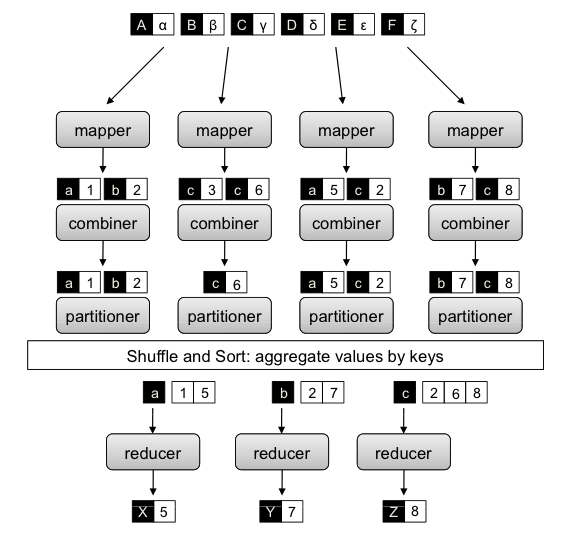
\includegraphics[scale=0.4]{./Figures/combiners}
    \end{center}
}

%%%%%%%%%%%%%%%%%%%%%%%%%%%%%%%%%%%%%%%%%%%%%%%%%%%%%%%%%%
\frame {\frametitle{Word Counting in MapReduce}
%%%%%%%%%%%%%%%%%%%%%%%%%%%%%%%%%%%%%%%%%%%%%%%%%%%%%%%%%%
   \begin{center}
   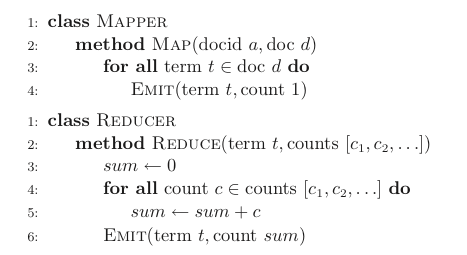
\includegraphics[scale=0.5]{./Figures/word_count}
    \end{center}
}

%%%%%%%%%%%%%%%%%%%%%%%%%%%%%%%%%%%%%%%%%%%%%%%%%%%%%%%%%%
\frame {\frametitle{In-Mapper Combiners}
%%%%%%%%%%%%%%%%%%%%%%%%%%%%%%%%%%%%%%%%%%%%%%%%%%%%%%%%%%
  \begin{itemize}
  \item \textbf{In-Mapper Combiners, a possible improvement}
    \begin{itemize}
    \item Hadoop does not guarantee combiners to be executed
    \end{itemize}

    \vspace{20pt}

  \item \textbf{Use an associative array to cumulate intermediate
      results}
    \begin{itemize}
    \item The array is used to tally up term counts within a single
      document
    \item The \texttt{Emit} method is called only after all
      \texttt{InputRecords} have been processed
    \end{itemize}

    \vspace{20pt}

  \item \textbf{Example (see next slide)}
    \begin{itemize}
    \item The code emits a key-value pair for each {\color{red}unique}
      term in the document
    \end{itemize}
  \end{itemize}
}

%%%%%%%%%%%%%%%%%%%%%%%%%%%%%%%%%%%%%%%%%%%%%%%%%%%%%%%%%%
\frame {\frametitle{In-Memory Combiners}
%%%%%%%%%%%%%%%%%%%%%%%%%%%%%%%%%%%%%%%%%%%%%%%%%%%%%%%%%%
   \begin{center}
   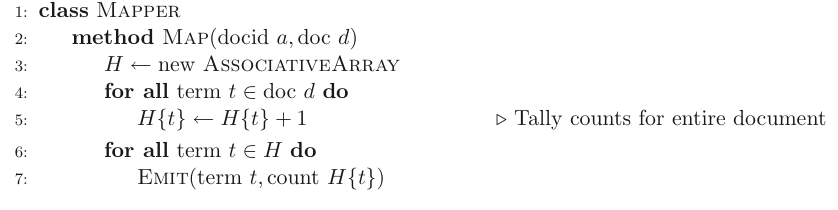
\includegraphics[scale=0.4]{./Figures/in_mapper_v1}
    \end{center}
}

\frame {\frametitle{In-Memory Combiners}
  \begin{itemize}
  \item \textbf{Taking the idea one step further}
    \begin{itemize}
    \item Exploit implementation details in Hadoop\footnote{Forward reference! We'll see more tomorrow.}
    \item A Java mapper object is created for each map task
    \item JVM reuse must be enabled
    \end{itemize}

    \vspace{40pt}

  \item \textbf{Preserve state within and across calls to the \texttt{Map}
    method}
    \begin{itemize}
    \item \texttt{Initialize} method, used to create a across-map persistent
      data structure
    \item \texttt{Close} method, used to emit intermediate key-value
      pairs only when all map task scheduled on one machine are done
    \end{itemize}
  \end{itemize}
}

%%%%%%%%%%%%%%%%%%%%%%%%%%%%%%%%%%%%%%%%%%%%%%%%%%%%%%%%%%
\frame {\frametitle{In-Memory Combiners}
%%%%%%%%%%%%%%%%%%%%%%%%%%%%%%%%%%%%%%%%%%%%%%%%%%%%%%%%%%
   \begin{center}
   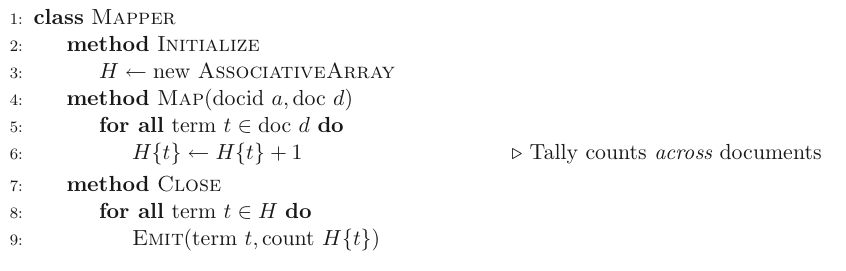
\includegraphics[scale=0.4]{./Figures/in_mapper_v2}
    \end{center}
}

%%%%%%%%%%%%%%%%%%%%%%%%%%%%%%%%%%%%%%%%%%%%%%%%%%%%%%%%%%
\frame {\frametitle{In-Memory Combiners}
%%%%%%%%%%%%%%%%%%%%%%%%%%%%%%%%%%%%%%%%%%%%%%%%%%%%%%%%%%
  \begin{itemize}
  \item \textbf{Summing up: a first ``design pattern'', \textit{in-memory
        combining}}
    \begin{itemize}
    \item Provides control over when local aggregation occurs
    \item Designer can determine how exactly aggregation is done
    \end{itemize}

    \vspace{40pt}

  \item \textbf{Efficiency vs. Combiners}
    \begin{itemize}
    \item There is no additional overhead due to the materialization
      of key-value pairs
      \begin{itemize}
      \item Un-necessary object creation and destruction (garbage
        collection)
      \item Serialization, deserialization when memory bounded
      \end{itemize}
    \item Mappers still need to emit all key-value pairs, combiners
      only reduce network traffic
    \end{itemize}
  \end{itemize}
}

%%%%%%%%%%%%%%%%%%%%%%%%%%%%%%%%%%%%%%%%%%%%%%%%%%%%%%%%%%
\frame {\frametitle{In-Memory Combiners}
%%%%%%%%%%%%%%%%%%%%%%%%%%%%%%%%%%%%%%%%%%%%%%%%%%%%%%%%%%
  \begin{itemize}
  \item \textbf{Precautions}
    \begin{itemize}
    \item In-memory combining breaks the functional programming
      paradigm due to state preservation
    \item Preserving state across multiple instances implies that
      algorithm behavior might depend on execution order
      \begin{itemize}
      \item Ordering-dependent bugs are difficult to find
      \end{itemize}
    \end{itemize}

    \vspace{20pt}

  \item \textbf{Scalability bottleneck}
    \begin{itemize}
    \item The in-memory combining technique strictly depends on having
      sufficient memory to store intermediate results
      \begin{itemize}
      \item And you don't want the OS to deal with swapping
      \end{itemize}
    \item Multiple threads compete for the same resources
    \item A possible {\color{red}solution}: ``block'' and ``flush''
      \begin{itemize}
      \item Implemented with a simple counter
      \end{itemize}
    \end{itemize}
  \end{itemize}
}

%%%%%%%%%%%%%%%%%%%%%%%%%%%%%%%%%%%%%%%%%%%%%%%%%%%%%%%%%%
\frame {\frametitle{Further Remarks}
%%%%%%%%%%%%%%%%%%%%%%%%%%%%%%%%%%%%%%%%%%%%%%%%%%%%%%%%%%
  \begin{itemize}
  \item \textbf{The extent to which efficiency can be increased with local
      aggregation depends on the size of the intermediate key space}
    \begin{itemize}
    \item Opportunities for aggregation arise when multiple values
      are associated to the same keys
    \end{itemize}

    \vspace{40pt}

  \item \textbf{Local aggregation also effective to deal with reduce
      stragglers}
    \begin{itemize}
    \item Reduce the number of values associated with frequently
      occuring keys
    \end{itemize}
  \end{itemize}
}

%%%%%%%%%%%%%%%%%%%%%%%%%%%%%%%%%%%%%%%%%%%%%%%%%%%%%%%%%%
\frame {\frametitle{Algorithmic correctness with local aggregation}
%%%%%%%%%%%%%%%%%%%%%%%%%%%%%%%%%%%%%%%%%%%%%%%%%%%%%%%%%%
  \begin{itemize}
  \item \textbf{The use of combiners must be thought carefully}
    \begin{itemize}
    \item In Hadoop, they are optional: the correctness of the
      algorithm cannot depend on computation (or even execution) of
      the combiners
    \end{itemize}

    \vspace{20pt}

  \item \textbf{In MapReduce, the reducer input key-value type must match the
      mapper output key-value type}
    \begin{itemize}
    \item Hence, for combiners, both input and output key-value types
      must match the output key-value type of the mapper
    \end{itemize}

    \vspace{20pt}

  \item \textbf{Commutative and Associative computations}
    \begin{itemize}
    \item This is a special case, which worked for word counting
      \begin{itemize}
      \item There the combiner code is actually the reducer code
      \end{itemize}
    \item In general, combiners and reducers are not interchangeable
    \end{itemize}
  \end{itemize}
}

%%%%%%%%%%%%%%%%%%%%%%%%%%%%%%%%%%%%%%%%%%%%%%%%%%%%%%%%%%
\frame {\frametitle{Algorithmic Correctness: an Example}
%%%%%%%%%%%%%%%%%%%%%%%%%%%%%%%%%%%%%%%%%%%%%%%%%%%%%%%%%%
  \begin{itemize}
  \item \textbf{Problem statement}
    \begin{itemize}
    \item We have a large dataset where input keys are strings and input
      values are integers
    \item We wish to compute the mean of all integers associated with
      the same key
      \begin{itemize}
      \item In practice: the dataset can be a log from a website,
        where the keys are user IDs and values are some measure of activity
      \end{itemize}
    \end{itemize}

    \vspace{20pt}

  \item \textbf{Next, a baseline approach}
    \begin{itemize}
    \item We use an \textbf{identity mapper}, which groups and sorts
      appropriately input key-value pairs
    \item Reducers keep track of running sum and the number of
      integers encountered
    \item The mean is emitted as the output of the reducer, with the
      input string as the key
    \end{itemize}

    \vspace{20pt}

  \item \textbf{Inefficiency problems in the shuffle phase}
  \end{itemize}
}

%%%%%%%%%%%%%%%%%%%%%%%%%%%%%%%%%%%%%%%%%%%%%%%%%%%%%%%%%%
\frame {\frametitle{Example: basic way to compute the mean of values}
%%%%%%%%%%%%%%%%%%%%%%%%%%%%%%%%%%%%%%%%%%%%%%%%%%%%%%%%%%
   \begin{center}
   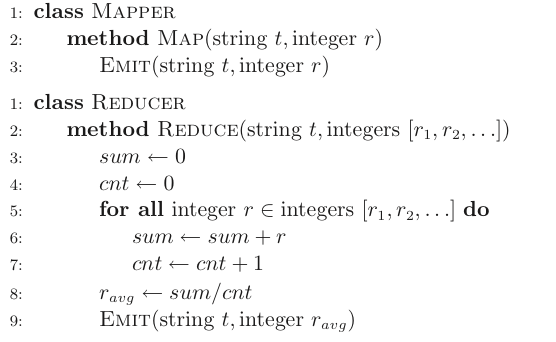
\includegraphics[scale=0.4]{./Figures/average_v1}
    \end{center}
}

%%%%%%%%%%%%%%%%%%%%%%%%%%%%%%%%%%%%%%%%%%%%%%%%%%%%%%%%%%
\frame {\frametitle{Algorithmic Correctness}
%%%%%%%%%%%%%%%%%%%%%%%%%%%%%%%%%%%%%%%%%%%%%%%%%%%%%%%%%%
  \begin{itemize}
  \item \textbf{Note: operations are not distributive}
    \begin{itemize}
    \item \texttt{Mean}(1,2,3,4,5) $\neq$
      \texttt{Mean}(\texttt{Mean}(1,2), \texttt{Mean}(3,4,5))
    \item Hence: a combiner cannot output partial means and hope that
      the reducer will compute the correct final mean
    \end{itemize}

    \vspace{20pt}

  \item \textbf{Next, a failed attempt at solving the problem}
    \begin{itemize}
    \item The combiner partially aggregates results by separating the
      components to arrive at the mean
    \item The sum and the count of elements are packaged into a pair
    \item Using the same input string, the combiner emits the pair
    \end{itemize}
  \end{itemize}
}

%%%%%%%%%%%%%%%%%%%%%%%%%%%%%%%%%%%%%%%%%%%%%%%%%%%%%%%%%%
\frame {\frametitle{Example: {\color{red}Wrong} use of combiners}
%%%%%%%%%%%%%%%%%%%%%%%%%%%%%%%%%%%%%%%%%%%%%%%%%%%%%%%%%%
   \begin{center}
   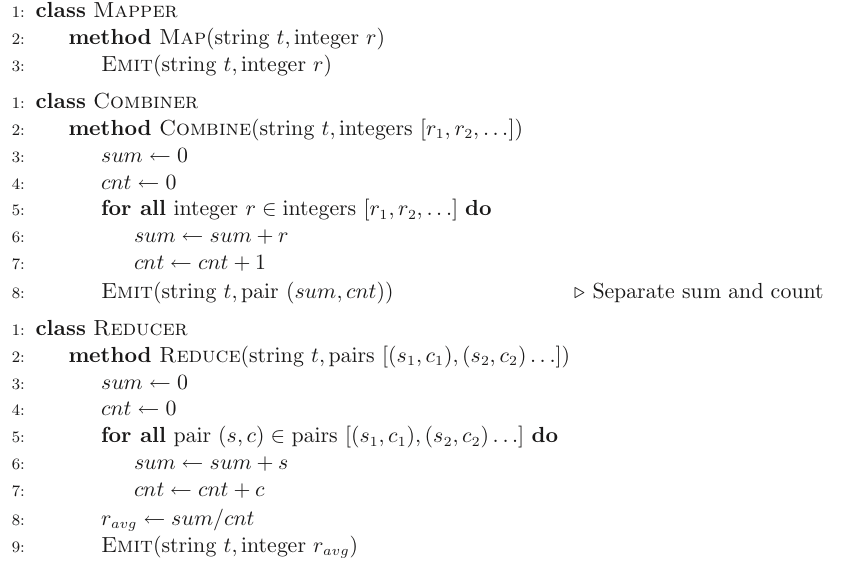
\includegraphics[scale=0.35]{./Figures/average_v2}
    \end{center}
}

%%%%%%%%%%%%%%%%%%%%%%%%%%%%%%%%%%%%%%%%%%%%%%%%%%%%%%%%%%
\frame {\frametitle{Algorithmic Correctness: an Example}
%%%%%%%%%%%%%%%%%%%%%%%%%%%%%%%%%%%%%%%%%%%%%%%%%%%%%%%%%%
  \begin{itemize}
  \item \textbf{What's wrong with the previous approach?}
    \begin{itemize}
    \item {\color{red}Trivially}, the input/output keys are not
      correct
    \item Remember that combiners are optimizations, the algorithm
      should work even when ``removing'' them
    \end{itemize}

    \vspace{20pt}

  \item \textbf{Executing the code omitting the combiner phase}
    \begin{itemize}
    \item The output value type of the mapper is integer
    \item The reducer expects to receive a list of integers
    \item Instead, we make it expect a list of pairs
    \end{itemize}

    \vspace{20pt}
    

  \item \textbf{Next, a correct implementation of the combiner}
    \begin{itemize}
    \item Note: the reducer is similar to the combiner!
    \item Exercise: verify the correctness
    \end{itemize}
  \end{itemize}
}

%%%%%%%%%%%%%%%%%%%%%%%%%%%%%%%%%%%%%%%%%%%%%%%%%%%%%%%%%%
\frame {\frametitle{Example: {\color{red}Correct} use of combiners}
%%%%%%%%%%%%%%%%%%%%%%%%%%%%%%%%%%%%%%%%%%%%%%%%%%%%%%%%%%
   \begin{center}
   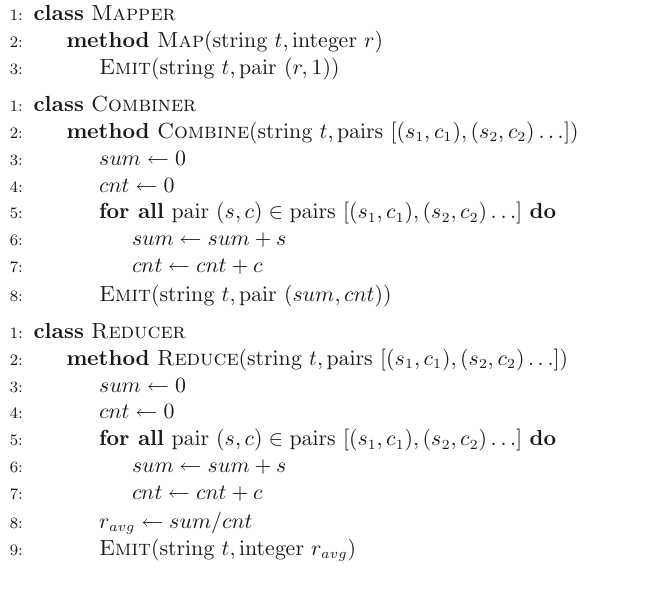
\includegraphics[scale=0.35]{./Figures/average_v3}
    \end{center}
}

%%%%%%%%%%%%%%%%%%%%%%%%%%%%%%%%%%%%%%%%%%%%%%%%%%%%%%%%%%
\frame {\frametitle{Advanced technique}
%%%%%%%%%%%%%%%%%%%%%%%%%%%%%%%%%%%%%%%%%%%%%%%%%%%%%%%%%%
  \begin{itemize}
  \item \textbf{Using in-mapper combining}
    \begin{itemize}
    \item Inside the mapper, the partial sums and counts are
      held in memory (across inputs)
    \item Intermediate values are emitted only after the entire input
      split is processed
    \item Similarly to before, the output value is a pair
    \end{itemize}
  \end{itemize}

   \begin{center}
   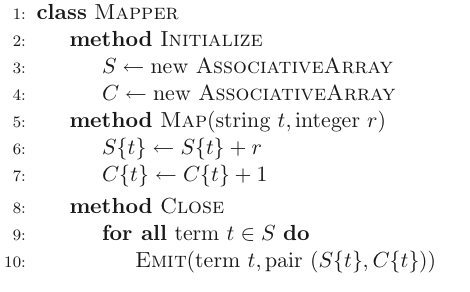
\includegraphics[scale=0.4]{./Figures/average_v4}
    \end{center}

} 

%%%%%%%%%%%%%%%%%%%%%%%%%%%%%%%%%%%%%%%%%%%%%%%%%%%%%%%%%%
%%%%%%%%%%%%%%%%%%%%%%%%%%%%%%%%%%%%%%%%%%%%%%%%%%%%%%%%%%
\subsection{Pairs and Stripes}
%%%%%%%%%%%%%%%%%%%%%%%%%%%%%%%%%%%%%%%%%%%%%%%%%%%%%%%%%%
%%%%%%%%%%%%%%%%%%%%%%%%%%%%%%%%%%%%%%%%%%%%%%%%%%%%%%%%%%

%%%%%%%%%%%%%%%%%%%%%%%%%%%%%%%%%%%%%%%%%%%%%%%%%%%%%%%%%%
\frame {\frametitle{Pairs and Stripes}
%%%%%%%%%%%%%%%%%%%%%%%%%%%%%%%%%%%%%%%%%%%%%%%%%%%%%%%%%%
  \begin{itemize}
  \item \textbf{A common approach in MapReduce: build
      {\color{red}complex} keys}
    \begin{itemize}
    \item Data necessary for a computation are naturally brought
      together by the framework
    \end{itemize}

    \vspace{20pt}

  \item \textbf{Two basic techniques:}
   \begin{itemize}
    \item \textit{Pairs}: similar to the example on the average
    \item \textit{Stripes}: uses in-mapper memory data structures
    \end{itemize}

    \vspace{20pt}

  \item \textbf{Next, we focus on a particular problem that benefits
      from these two methods}
 \end{itemize}
}

%%%%%%%%%%%%%%%%%%%%%%%%%%%%%%%%%%%%%%%%%%%%%%%%%%%%%%%%%%
\frame {\frametitle{Problem statement}
%%%%%%%%%%%%%%%%%%%%%%%%%%%%%%%%%%%%%%%%%%%%%%%%%%%%%%%%%%
  \begin{itemize}
  \item \textbf{The problem: building word co-occurrence matrices for
      large corpora}
    \begin{itemize}
    \item The co-occurrence matrix of a corpus is a square $n \times
      n$ matrix
    \item $n$ is the number of unique words (\textit{i.e.}, the
      vocabulary size)
    \item A cell $m_{ij}$ contains the number of times the word $w_i$
      co-occurs with word $w_j$ \textit{within a specific context}
    \item Context: a sentence, a paragraph a document or a window of
      $m$ words
    \item NOTE: the matrix may be symmetric in some cases
    \end{itemize}

    \vspace{20pt}

  \item \textbf{Motivation}
    \begin{itemize}
    \item This problem is a basic building block for more complex
      operations
    \item {\color{red}Estimating the distribution of discrete
        joint events from a large number of observations}
    \item Similar problem in other domains:
      \begin{itemize}
      \item Customers who buy \textit{this} tend to also buy
        \textit{that}
      \end{itemize}
    \end{itemize}
  \end{itemize}
}

%%%%%%%%%%%%%%%%%%%%%%%%%%%%%%%%%%%%%%%%%%%%%%%%%%%%%%%%%%
\frame {\frametitle{Observations}
%%%%%%%%%%%%%%%%%%%%%%%%%%%%%%%%%%%%%%%%%%%%%%%%%%%%%%%%%%
  \begin{itemize}
  \item \textbf{Space requirements}
    \begin{itemize}
    \item Clearly, the space requirement is $O(n^2)$, where $n$ is the
      size of the vocabulary
    \item For real-world (English) corpora $n$ can be hundreds of
      thousands of words, or even billions of worlds in some specific cases
    \end{itemize}

    \vspace{20pt}

  \item \textbf{So what's the problem?}
    \begin{itemize}
    \item If the matrix can fit in the memory of a single machine,
      then just use whatever naive implementation
    \item Instead, if the matrix is bigger than the available memory,
      then {\color{red}paging} would kick in, and any naive
      implementation would break
    \end{itemize}

    \vspace{20pt}

  \item \textbf{Compression}
    \begin{itemize}
    \item Such techniques can help in solving the problem on a single
      machine
    \item However, there are scalability problems
    \end{itemize}
  \end{itemize}
}

%%%%%%%%%%%%%%%%%%%%%%%%%%%%%%%%%%%%%%%%%%%%%%%%%%%%%%%%%%
\frame {\frametitle{Word co-occurrence: the Pairs approach}
%%%%%%%%%%%%%%%%%%%%%%%%%%%%%%%%%%%%%%%%%%%%%%%%%%%%%%%%%%
  \begin{itemize}
  \item \textbf{Input to the problem}
    \begin{itemize}
    \item Key-value pairs in the form of a \texttt{docid} and a \texttt{doc}
    \end{itemize}

    \vspace{20pt}

  \item \textbf{The mapper:}
    \begin{itemize}
    \item Processes each input document
      \item Emits key-value pairs with:
        \begin{itemize}
        \item Each co-occurring word {\color{red}pair} as the key
        \item The integer one (the count) as the value
        \end{itemize}
      \item This is done with two nested loops:
        \begin{itemize}
        \item The outer loop iterates over all words
        \item The inner loop iterates over all neighbors
        \end{itemize}
    \end{itemize}

    \vspace{20pt}

  \item \textbf{The reducer:}
    \begin{itemize}
    \item Receives {\color{red}pairs} related to co-occurring words
      \begin{itemize}
      \item This {\color{red}requires \textbf{modifying the partitioner}}
      \end{itemize}
    \item Computes an absolute count of the joint event
    \item Emits the pair and the count as the final key-value output
      \begin{itemize}
      \item Basically reducers emit the cells of the output matrix
      \end{itemize}
    \end{itemize}
  \end{itemize}
}

%%%%%%%%%%%%%%%%%%%%%%%%%%%%%%%%%%%%%%%%%%%%%%%%%%%%%%%%%%
\frame {\frametitle{Word co-occurrence: the Pairs approach}
%%%%%%%%%%%%%%%%%%%%%%%%%%%%%%%%%%%%%%%%%%%%%%%%%%%%%%%%%%
  \begin{center}
    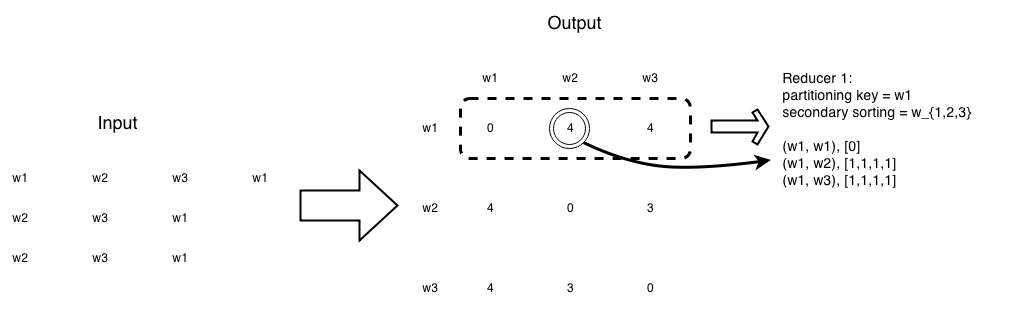
\includegraphics[scale=0.4]{./Figures/pairs}
  \end{center}
}

%%%%%%%%%%%%%%%%%%%%%%%%%%%%%%%%%%%%%%%%%%%%%%%%%%%%%%%%%%
\frame {\frametitle{Word co-occurrence: the Stripes approach}
%%%%%%%%%%%%%%%%%%%%%%%%%%%%%%%%%%%%%%%%%%%%%%%%%%%%%%%%%%
  \begin{itemize}
  \item \textbf{Input to the problem}
    \begin{itemize}
    \item Key-value pairs in the form of a \texttt{docid} and a \texttt{doc}
    \end{itemize}

    \vspace{20pt}

  \item \textbf{The mapper:}
    \begin{itemize}
    \item Same two nested loops structure as before
    \item Co-occurrence information is first stored in an associative
      array
    \item Emit key-value pairs with {\color{red}words} as keys and the
      corresponding arrays as values
    \end{itemize}

    \vspace{20pt}

  \item \textbf{The reducer:}
    \begin{itemize}
    \item Receives all associative arrays related to the same word
    \item Performs an element-wise sum of all associative arrays with
      the same key
    \item Emits key-value output in the form of word, associative
      array
      \begin{itemize}
      \item Basically, reducers emit \textbf{rows} of the co-occurrence matrix
      \end{itemize}
    \end{itemize}
 \end{itemize}

}

%%%%%%%%%%%%%%%%%%%%%%%%%%%%%%%%%%%%%%%%%%%%%%%%%%%%%%%%%%
\frame {\frametitle{Word co-occurrence: the Stripes approach}
%%%%%%%%%%%%%%%%%%%%%%%%%%%%%%%%%%%%%%%%%%%%%%%%%%%%%%%%%%
  \begin{center}
    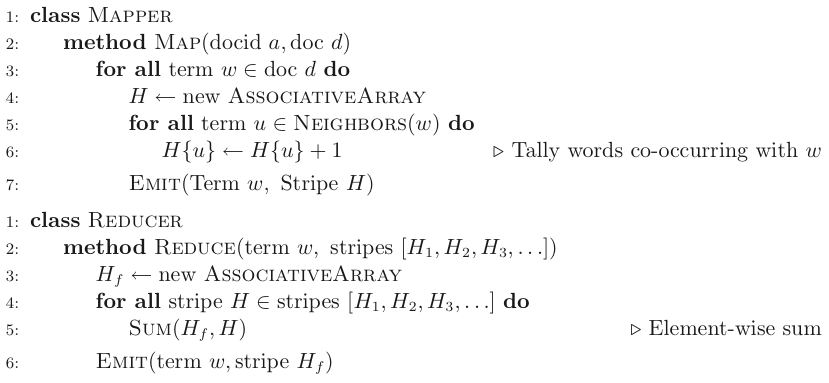
\includegraphics[scale=0.4]{./Figures/stripes}
  \end{center}
}

%%%%%%%%%%%%%%%%%%%%%%%%%%%%%%%%%%%%%%%%%%%%%%%%%%%%%%%%%%
\frame {\frametitle{Pairs and Stripes, a comparison}
%%%%%%%%%%%%%%%%%%%%%%%%%%%%%%%%%%%%%%%%%%%%%%%%%%%%%%%%%%
  \begin{itemize}
  \item \textbf{The pairs approach}
    \begin{itemize}
    \item Generates a large number of key-value pairs
    \begin{itemize}
      \item In particular, intermediate ones, that fly over the network
    \end{itemize}
    \item The benefit from combiners is limited, as it is less likely
      for a mapper to process multiple occurrences of a word
    \item Does not suffer from memory paging problems
    \end{itemize}

    \vspace{20pt}
    
  \item \textbf{The stripes approach}
    \begin{itemize}
    \item More compact
    \item Generates fewer and shorted intermediate keys
      \begin{itemize}
      \item The framework has less sorting to do
      \end{itemize}
    \item The values are more complex and have
      serialization/deserialization overhead
    \item Greatly benefits from combiners, as the key space is the
      vocabulary
    \item Suffers from memory paging problems, if not properly engineered
    \end{itemize}
  \end{itemize}
}

%%%%%%%%%%%%%%%%%%%%%%%%%%%%%%%%%%%%%%%%%%%%%%%%%%%%%%%%%%
%%%%%%%%%%%%%%%%%%%%%%%%%%%%%%%%%%%%%%%%%%%%%%%%%%%%%%%%%%
\subsection{Order Inversion}
%%%%%%%%%%%%%%%%%%%%%%%%%%%%%%%%%%%%%%%%%%%%%%%%%%%%%%%%%%
%%%%%%%%%%%%%%%%%%%%%%%%%%%%%%%%%%%%%%%%%%%%%%%%%%%%%%%%%%

%%%%%%%%%%%%%%%%%%%%%%%%%%%%%%%%%%%%%%%%%%%%%%%%%%%%%%%%%%
\frame {\frametitle{Computing relative frequencies}
%%%%%%%%%%%%%%%%%%%%%%%%%%%%%%%%%%%%%%%%%%%%%%%%%%%%%%%%%%
  \begin{itemize}
  \item \textbf{``Relative'' Co-occurrence matrix construction}
    \begin{itemize}
    \item Similar problem as before, same matrix
    \item Instead of absolute counts, we take into consideration the
      fact that some words appear more frequently than others
      \begin{itemize}
      \item Word $w_i$ may co-occur frequently with word $w_j$ simply
        because one of the two is very common
      \end{itemize}
    \item We need to convert absolute counts to relative frequencies
      $f(w_j | w_i)$
      \begin{itemize}
      \item What proportion of the time does $w_j$ appear in the
        context of $w_i$?
      \end{itemize}
    \end{itemize}

    \vspace{20pt}

  \item \textbf{Formally, we compute:}
    $$ f(w_j | w_i) = \frac{N(w_i,w_j)}{\sum_{w'} N(w_i, w')}$$
    \begin{itemize}
    \item $N(\cdot,\cdot)$ is the number of times a co-occurring word
      pair is observed
    \item The denominator is called the marginal
    \end{itemize}


  \end{itemize}
}

%%%%%%%%%%%%%%%%%%%%%%%%%%%%%%%%%%%%%%%%%%%%%%%%%%%%%%%%%%
\frame {\frametitle{Computing relative frequencies}
%%%%%%%%%%%%%%%%%%%%%%%%%%%%%%%%%%%%%%%%%%%%%%%%%%%%%%%%%%
  \begin{itemize}
  \item \textbf{The stripes approach}
    \begin{itemize}
    \item In the reducer, the counts of all words that co-occur with
      the conditioning variable ($w_i$) are available in the
      associative array
    \item Hence, the sum of all those counts gives the marginal
    \item Then we divide the the joint counts by the marginal and
      we're done
    \end{itemize}

    \vspace{40pt}

  \item \textbf{The pairs approach}
    \begin{itemize}
    \item The reducer receives the pair $(w_i,w_j)$ and the count
    \item From this information alone \textbf{it is not possible} to compute
      $f(w_j | w_i)$
    \item Fortunately, as for the mapper, also the reducer can
      {\color{red}preserve state} across multiple keys
      \begin{itemize}
      \item We can buffer in memory all the words that co-occur with
        $w_i$ and their counts
      \item This is basically building the associative array in the
        stripes method
      \end{itemize}
    \end{itemize}
  \end{itemize}
}

%%%%%%%%%%%%%%%%%%%%%%%%%%%%%%%%%%%%%%%%%%%%%%%%%%%%%%%%%%
\frame {\frametitle{Computing relative frequencies: a basic approach}
%%%%%%%%%%%%%%%%%%%%%%%%%%%%%%%%%%%%%%%%%%%%%%%%%%%%%%%%%%
  \begin{itemize}
  \item \textbf{We must define the sort order of the pair}
    \begin{itemize}
    \item In this way, the keys are first sorted by the left word, and
      then by the right word (in the pair)
    \item Hence, we can detect if  all pairs associated with the word
      we are conditioning on ($w_i$) have been seen
    \item At this point, we can use the in-memory buffer, compute the
      relative frequencies and emit
    \end{itemize}

    \vspace{20pt}

  \item \textbf{We must define an appropriate partitioner}
    \begin{itemize}
    \item The default partitioner is based on the hash value of the
      intermediate key, modulo the number of reducers
    \item For a complex key, the raw byte representation is used to
      compute the hash value
      \begin{itemize}
      \item Hence, there is no guarantee that the pair (dog, aardvark)
        and (dog,zebra) are sent to the same reducer
      \end{itemize}
    \item What we want is that all pairs with the same left word are
      sent to the same reducer
   \end{itemize}

    \vspace{20pt}

  \item \textbf{Limitations of this approach}
    \begin{itemize}
    \item Essentially, we reproduce the stripes method on the reducer
      and we need to use a custom partitioner
    \item This algorithm would work, but present the same
      memory-bottleneck problem as the stripes method
    \end{itemize}
  \end{itemize}
}

%%%%%%%%%%%%%%%%%%%%%%%%%%%%%%%%%%%%%%%%%%%%%%%%%%%%%%%%%%
\frame {\frametitle{Computing relative frequencies: order inversion}
%%%%%%%%%%%%%%%%%%%%%%%%%%%%%%%%%%%%%%%%%%%%%%%%%%%%%%%%%%
  \begin{itemize}
  \item \textbf{The key is to properly sequence data presented to
      reducers}
    \begin{itemize}
    \item If it were possible to compute the marginal in the reducer
      before processing the joint counts, the reducer could simply
      divide the joint counts received from mappers by the marginal
    \item The notion of ``before'' and ``after'' can be captured in
      the {\color{red}ordering of key-value pairs}
    \item The programmer can define the sort order of keys so that
      data needed earlier is presented to the reducer before data that
      is needed later
    \end{itemize}
\end{itemize}
}

%%%%%%%%%%%%%%%%%%%%%%%%%%%%%%%%%%%%%%%%%%%%%%%%%%%%%%%%%%
\frame {\frametitle{Computing relative frequencies: order inversion}
%%%%%%%%%%%%%%%%%%%%%%%%%%%%%%%%%%%%%%%%%%%%%%%%%%%%%%%%%%
  \begin{itemize}
  \item \textbf{Recall that mappers emit pairs of co-occurring words
      as keys}

    \vspace{20pt}

  \item \textbf{The mapper:}
    \begin{itemize}
    \item additionally emits a ``special'' key of the form $(w_i,*)$
    \item The value associated to the special key is one, that
      represents the contribution of the word pair to the marginal
    \item Using combiners, these partial marginal counts will be
      aggregated before being sent to the reducers
    \end{itemize}

    \vspace{20pt}

  \item \textbf{The reducer:}
    \begin{itemize}
    \item We must make sure that the special key-value pairs are
      processed {\color{red}before} any other key-value pairs where
      the left word is $w_i$
    \item We also need to modify the partitioner as before,
      \textit{i.e.}, it would take into account only the first word
    \end{itemize}
  \end{itemize}
}


%%%%%%%%%%%%%%%%%%%%%%%%%%%%%%%%%%%%%%%%%%%%%%%%%%%%%%%%%%
\frame {\frametitle{Computing relative frequencies: order inversion}
%%%%%%%%%%%%%%%%%%%%%%%%%%%%%%%%%%%%%%%%%%%%%%%%%%%%%%%%%%
  \begin{itemize}
  \item \textbf{Memory requirements:}
    \begin{itemize}
    \item Minimal, because only the marginal (an integer) needs to be
      stored
    \item No buffering of individual co-occurring word
    \item No scalability bottleneck
    \end{itemize}

    \vspace{20pt}

  \item \textbf{Key ingredients for order inversion}
    \begin{itemize}
    \item Emit a special key-value pair to capture the marginal
    \item Control the sort order of the intermediate key, so that the
      special key-value pair is processed first
    \item Define a custom partitioner for routing intermediate
      key-value pairs
    \item Preserve state across multiple keys in the reducer
    \end{itemize}
  \end{itemize}
}
